\documentclass[fleqn]{article}
\usepackage[spanish]{babel}
\usepackage{amsmath, amssymb, amsfonts}
\usepackage{parskip, nopageno}
\usepackage[a4paper, margin = 2.1cm]{geometry}
\usepackage{graphicx, subfigure}
\usepackage[p,osf]{scholax}
\usepackage[scaled=1.075,ncf,vvarbb]{newtxmath}

\begin{document}
    \begin{center}
        {\Huge \textbf{Regiones elementales y sus fronteras}} 
    \end{center}
    \vspace{7mm}

    \textbf{Region elemental (en $ \mathbb{R}^3 $):} Es aquella en la que una de las variables esta acotada, inferior y superiormente, por funciones, $ \gamma_1 $ y $ \gamma_2 $ (donde $ \gamma_2 \geq \gamma_1 $), que dependen de las otras dos variables y su dominio es una región elemental en $ \mathbb{R}^2 $. 

    Por ejemplo:

    \begin{enumerate}

        \item $ W = \left\lbrace (x,y,z) \in \mathbb{R}^3 \; \big| \; 0 \leq x \leq \sqrt{2}, 0 \leq y \leq \sqrt{2 - x^2} \text{ y } x^2 + y^2 \leq z \leq 2 \right\rbrace $
        
        \begin{figure}[htb]
            \centering
            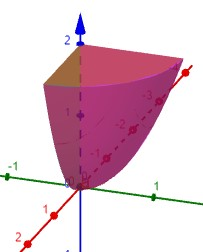
\includegraphics{Captura_1.jpg}
        \end{figure}

    \end{enumerate}

    \textbf{Superficie cerrada:} Sea $ W $ una región elemental en $ \mathbb{R}^3 $. A $ \partial W $ se le llama superficie cerrada. Las superficies $ S_1, S_2, \dots , S_6 $ que conforman a $ \partial W $, tales que pueden representarse como gráficas de funciones de $ \mathbb{R}^2 $ a $ \mathbb{R} $, son sus caras.

    Por ejemplo, considerando la región $ W $ del ejemplo anterior, sus caras son:

    \begin{itemize}
        \item $ S_1 $ es la gráfica de la función $ f_1 : D_1 \subset \mathbb{R}^2 \to \mathbb{R} $ donde $ D_1 = \left\lbrace (x,z) \in \mathbb{R}^2 \; \big| \; 0 \leq x \leq \sqrt{2} \text{ y } x^2 \leq z \leq 2 \right\rbrace $ y $ f_1(x,z) = 0 $.

        \item $ S_2 $ es la gráfica de la función $ f_2 : D_2 \subset \mathbb{R}^2 \to \mathbb{R} $ donde $ D_2 = \left\lbrace (y,z) \in \mathbb{R}^2 \; \big| \; 0 \leq y \leq \sqrt{2} \text{ y } y^2 \leq z \leq 2 \right\rbrace $ y $ f_2(y,z) = 0 $.

        \item $ S_3 $ es la gráfica de la función $ f_3 : D_3 \subset \mathbb{R}^2 \to \mathbb{R} $ donde $ D_3 = \left\lbrace (x,y) \in \mathbb{R}^2 \; \big| \; 0 \leq x \leq \sqrt{2} \text{ y } 0 \leq y \leq \sqrt{2 - x^2} \right\rbrace $ y $ f_3(x,y) = 2 $.

        \item $ S_4 $ es la gráfica de la función $ f_4 : D_4 \subset \mathbb{R}^2 \to \mathbb{R} $ donde $ D_4 = \left\lbrace (x,y) \in \mathbb{R}^2 \; \big| \; 0 \leq x \leq \sqrt{2} \text{ y } 0 \leq y \leq \sqrt{2 - x^2} \right\rbrace $ y $ f_4(x,y) = x^2 + y^2 $.

        \begin{figure}[htbp]
            \centering
            \subfigure[$ S_1 $]{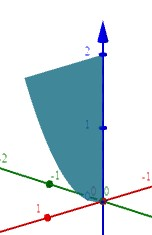
\includegraphics[width=30mm]{./Captura_2.jpg}}
            \subfigure[$ S_2 $]{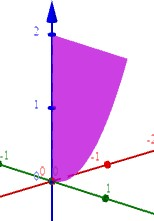
\includegraphics[width=30mm]{./Captura_3.jpg}}
            \subfigure[$ S_3 $]{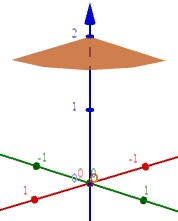
\includegraphics[width=30mm]{./Captura_4.jpg}}
            \subfigure[$ S_4 $]{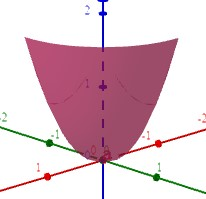
\includegraphics[width=30mm]{./Captura_5.jpg}}
        \end{figure}
    \end{itemize}

    \textbf{Definición:} Sea $ S $ una superficie cerrada. 

    \begin{itemize}
        \item Si el vector normal a $ S $ apunta al exterior de este, entonces la superficie tiene orientación exterior. 
        \item Si el vector normal a $ S $ apunta al interior de este, entonces la superficie tiene orientación interior.
    \end{itemize}
    
    Sea $ \overrightarrow{F}  $ el campo de velocidades de un fluido. 

    \begin{itemize}
        \item Si $ S $ tiene orientación exterior entonces $ \displaystyle \iint_S \overrightarrow{F} \cdot \mathrm{d} \overrightarrow{s} $ representa la cantidad de fluido que sale de $ S $ por unidad de tiempo.
        
        \item Si $ S $ tiene orientación interior entonces $ \displaystyle \iint_S \overrightarrow{F} \cdot \mathrm{d} \overrightarrow{s} $ representa la cantidad de fluido que atraviesa $ S $ hacia el interior, por unidad de tiempo.
    \end{itemize}

    Ahora, sea $ n(x,y,z) $ un vector normal unitario que representa la orientación de $ S $. Se sabe que

    $ \displaystyle \iint_S \overrightarrow{F} \cdot \mathrm{d} \overrightarrow{s} = \displaystyle \iint_S \left(\overrightarrow{F} \cdot n \right) \mathrm{d} s $

    Se adoptará el convenio de que una superficie cerrada $ S $, tal que $ S = \partial W $, para una región elemental $ W $, tiene orientación exterior unitaria $ n(x,y,z) $ para cada $ (x,y,z) \in S $. Además, se denotará a la misma superficie, pero con orientación interior, como $ \partial W_{op} $. Así,

    $ \displaystyle \iint_{\partial W} \overrightarrow{F} \cdot \mathrm{d} \overrightarrow{s} = \displaystyle \iint_S \left(\overrightarrow{F} \cdot n \right) \mathrm{d} s = - \displaystyle \iint_S \left[\overrightarrow{F} \cdot (-n) \right] \mathrm{d} s = \displaystyle \iint_{\partial W_{op}} \overrightarrow{F} \cdot \mathrm{d} \overrightarrow{s} $.

    Ejemplo:

    Sea $ W = \left\lbrace (x,y,z) \in \mathbb{R}^3 \; \big| \; 0 \leq x \leq 1, 0 \leq y \leq 1 \text{ y } 0 \leq z \leq 1 \right\rbrace $ el cubo unitario. Cada una de sus caras se pueden escribir como sigue:

    $ S_1 = \left\lbrace (x,y,z) \in \mathbb{R}^3 \; \big| \; 0 \leq x \leq 1, 0 \leq y \leq 1 \text{ y } z = 0 \right\rbrace $,

    $ S_2 = \left\lbrace (x,y,z) \in \mathbb{R}^3 \; \big| \; 0 \leq x \leq 1, 0 \leq y \leq 1 \text{ y } z = 1 \right\rbrace $,

    $ S_3 = \left\lbrace (x,y,z) \in \mathbb{R}^3 \; \big| \; 0 \leq y \leq 1, 0 \leq z \leq 1 \text{ y } x = 0 \right\rbrace $,

    $ S_4 = \left\lbrace (x,y,z) \in \mathbb{R}^3 \; \big| \; 0 \leq y \leq 1, 0 \leq z \leq 1 \text{ y } x = 1 \right\rbrace $,

    $ S_5 = \left\lbrace (x,y,z) \in \mathbb{R}^3 \; \big| \; 0 \leq x \leq 1, 0 \leq z \leq 1 \text{ y } y = 0 \right\rbrace $ y

    $ S_6 = \left\lbrace (x,y,z) \in \mathbb{R}^3 \; \big| \; 0 \leq x \leq 1, 0 \leq z \leq 1 \text{ y } y = 1 \right\rbrace $.

    \begin{figure}[htb]
        \centering
        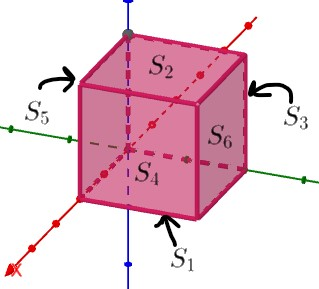
\includegraphics{Caotura 6.jpg}
    \end{figure}

    De esta manera, para un campo vectorial continuo $ F = F_1 \widehat{i} + F_2 \widehat{j} + F_3 \widehat{k} $, se tiene que

    $ \displaystyle \iint_{\partial W} \overrightarrow{F} \cdot \mathrm{d} \overrightarrow{s} = \displaystyle \iint_S \left(\overrightarrow{F} \cdot n \right) \mathrm{d} s = - \displaystyle \iint_{S_1} F_3 \mathrm{d} s + \displaystyle \iint_{S_2} F_3 \mathrm{d} s - \displaystyle \iint_{S_3} F_1 \mathrm{d} s + \displaystyle \iint_{S_4} F_1 \mathrm{d} s - \displaystyle \iint_{S_5} F_2 \mathrm{d} s + \displaystyle \iint_{S_6} F_2 \mathrm{d} s $
\end{document}